\thispagestyle{empty} % Bỏ dấu trang

% Bìa 1 
\begin{center}
    % Tên trường     
    \textbf{\fontsize{15pt}{0pt}\selectfont TRƯỜNG ĐẠI HỌC BÁCH KHOA HÀ NỘI\\}

    % Vẽ đường thẳng 
    \vspace{-1.5ex}
    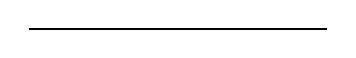
\begin{tikzpicture}
        \draw[thick] (0, 5cm) -- (3.79cm,5cm);
    \end{tikzpicture}
    
    % Chèn hình ảnh 
    \vspace{1em}
    \begin{figure}[H]
        \centering
        
\includegraphics[width=2.43cm, height=3.94cm]{image/Logo_Hust.png}
    \end{figure}
    
    % Tên Đồ án
    \vspace{1.5cm}
    {\sffamily \fontsize{21pt}{0pt}\selectfont {\textbf{ĐỒ ÁN TỐT NGHIỆP}}\\}
    \vspace{2em}
    {\sffamily \fontsize{17pt}{0pt}\selectfont {\textbf{THIẾT KẾ HỆ THỐNG TỰ ĐỘNG ĐIỀU CHỈNH NHIỆT ĐỘ TRONG THIẾT BỊ SẤY HOA QUẢ}}\\}
    % Tên 
    \vspace{2em}
    \textbf{\fontsize{11pt}{0pt}\selectfont LÊ ĐĂNG QUANG\\}
    \vspace{1ex}
    \fontsize{14pt}{0pt}\selectfont nguyenvanabc@sis.hust.edu.vn\\

    \vspace{1em}
    \textbf{\fontsize{14pt}{0pt}\selectfont Ngành KT Điều khiển \& Tự động hóa\\}
    \vspace{1ex}
    \textbf{\fontsize{14pt}{0pt}\selectfont Chuyên ngành Điều khiển tự động \\}

    % Bảng thông tin
    \vspace{5em}
    \begin{tabular}{  l  l  r }
        \textbf{Giảng viên hướng dẫn:}&PGS. TS. Phạm Văn ABC& \fontsize{10pt}{0pt}\selectfont \stackon{Chữ ký của GVHD}{\rule{4cm}{0.4pt}} \\ [3em] 
        \textbf{Bộ môn:}&Điều khiển tự động& \\ [1ex] 
        \textbf{Viện:}&Điện& \\
    \end{tabular}

    % Thời gian
    \vfill

    \textbf{HÀ NỘI, 12/2019}
\end{center}
% Bìa 2
\cleardoublepage
\thispagestyle{empty} % Bỏ dấu trang

\begin{center}
    % Tên trường     
    \textbf{\fontsize{15pt}{0pt}\selectfont TRƯỜNG ĐẠI HỌC BÁCH KHOA HÀ NỘI\\}

    % Vẽ đường thẳng 
    \vspace{-1.5ex}
    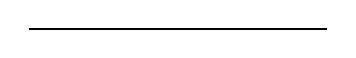
\begin{tikzpicture}
        \draw[thick] (0, 5cm) -- (3.79cm,5cm);
    \end{tikzpicture}
    
    % Chèn hình ảnh 
    \vspace{1em}
    \begin{figure}[H]
        \centering
        
\includegraphics[width=2.43cm, height=3.94cm]{image/Logo_Hust.png}
    \end{figure}
    
    % Tên Đồ án
    \vspace{1.5cm}
    {\sffamily \fontsize{21pt}{0pt}\selectfont {\textbf{ĐỒ ÁN TỐT NGHIỆP}}\\}
    \vspace{2em}
    {\sffamily \fontsize{17pt}{0pt}\selectfont {\textbf{THIẾT KẾ HỆ THỐNG TỰ ĐỘNG ĐIỀU CHỈNH NHIỆT ĐỘ TRONG THIẾT BỊ SẤY HOA QUẢ}}\\}
    % Tên 
    \vspace{2em}
    \textbf{\fontsize{11pt}{0pt}\selectfont LÊ ĐĂNG QUANG\\}
    \vspace{1ex}
    \fontsize{14pt}{0pt}\selectfont nguyenvanabc@sis.hust.edu.vn\\

    \vspace{1em}
    \textbf{\fontsize{14pt}{0pt}\selectfont Ngành KT Điều khiển \& Tự động hóa\\}
    \vspace{1ex}
    \textbf{\fontsize{14pt}{0pt}\selectfont Chuyên ngành Điều khiển tự động \\}

    % Bảng thông tin
    \vspace{5em}
    \begin{tabular}{  l  l  r }
        \textbf{Giảng viên hướng dẫn:}&PGS. TS. Phạm Văn ABC& \fontsize{10pt}{0pt}\selectfont \stackon{Chữ ký của GVHD}{\rule{4cm}{0.4pt}} \\ [3em] 
        \textbf{Bộ môn:}&Điều khiển tự động& \\ [1ex] 
        \textbf{Viện:}&Điện& \\
    \end{tabular}

    % Thời gian
    \vfill

    \textbf{HÀ NỘI, 12/2019}
\end{center}
\cleardoublepage
